%%%%%%%%%%%%%%%%%%%%%%%%%%%%%%%%%%%%%%%%%%%%%%%%%%%%%%%%%%%%%%%%%%%%%%%%%%%%%%%%
%% 实验报告模板.tex                                                           %%
%% author: hxp<hxp201406@gmail.com>                                           %%
%% 按照基础物理实验老师发的模板更改形成                                       %%
%%%%%%%%%%%%%%%%%%%%%%%%%%%%%%%%%%%%%%%%%%%%%%%%%%%%%%%%%%%%%%%%%%%%%%%%%%%%%%%%
%% 备注:刚刚的注释刚好是80行,编写代码的时候不要超过80行,就是你的代码不要超 %%
%% 过我注释里面最后面的“%”,超过请换行。                                      %%
%%%%%%%%%%%%%%%%%%%%%%%%%%%%%%%%%%%%%%%%%%%%%%%%%%%%%%%%%%%%%%%%%%%%%%%%%%%%%%%%
%% 模板现在开始,请根据注释把相应的位置更改成对应的内容                       %%
%%%%%%%%%%%%%%%%%%%%%%%%%%%%%%%%%%%%%%%%%%%%%%%%%%%%%%%%%%%%%%%%%%%%%%%%%%%%%%%%


\documentclass{ctexart}


\usepackage{ctex}
\usepackage{amsmath}
\usepackage{amsfonts}
\usepackage{amssymb}
\usepackage{wasysym}
\newcommand{\angstrom}{\text{\normalfont\AA}}  % 定义了原子物理的A
\usepackage{graphicx}
\usepackage{float}
\restylefloat{table}
\usepackage{geometry}
\geometry{a4paper,scale=0.8}  % 定义页面大小是A4,缩放是0.8
\usepackage{caption}
\usepackage{subcaption}
\usepackage{enumitem}

\newcommand*{\md}{\mathop{}\!\mathrm{d}}   % 定义微分算子,直立体的d
\newcommand*{\me}{\mathrm{e}}              % 定义自然对数e,同样应当是直立体

% 如果你想要每一段的开头不要空两格,注释掉下面这两行
% \usepackage{parskip}
% \setlength{\parindent}{0cm}

% 默认的\mathbf对希腊字母不生效,这里改下
\usepackage{bm}
\let\Oldmathbf\mathbf
\renewcommand{\mathbf}[1]{\boldsymbol{\Oldmathbf{#1}}}

% 表格默认格内内容和边框没有留出距离,显示分数的时候,分数的上下会贴到边框上
% 因此我增加了表格内容和边框的最短距离是5像素
\usepackage{cellspace}
\setlength{\cellspacetoplimit}{5pt}
\setlength{\cellspacebottomlimit}{5pt}

% \si命令是用来写单位的,单位需要和之前的数字有一个空格的距离,而且应当直立体
% 用法:5 \si{km/h}
\newcommand{\si}[1]{\  \mathrm{#1}}

% 日期不要显示
\date{}

\usepackage{fancyhdr}
\pagestyle{fancy}
\fancyhf{}
\lhead{本文档TeX源码地址:https://github.com/hxp-plus/Notes/tree/master/Physics-Experiment/实验报告}
\rfoot{第 \thepage 页}
\renewcommand{\headrulewidth}{1pt}
\renewcommand{\footrulewidth}{1pt}

%% 标题三号黑体,作者信息为班级姓名学号
\newcommand{\generatetitle}[6]{\title{\zihao{3}\heiti#1} \author{#2 \quad
    \quad #3 \quad\quad #4 \quad\quad #5 \quad\quad #6} \maketitle\thispagestyle{fancy}}

%% 所有的引言、实验内容与数据处理啥的,用section
\ctexset {
  section = {
    format = \raggedright\zihao{4}\heiti,  % 设置所有section的字号为四号黑体左对齐
    name={,、},                            % 序号后跟顿号
    aftername={\hspace{0pt}},              % 修改序号和标题直接的间距为零
    number=\chinese{section},              % 设置序号为中文
  },
  subsection = {
    format = \raggedright\zihao{5}\heiti,  % 设置所有subsection的字号为五号黑体左对齐
    number={},              % 设置序号为没有序号
  },
  subsubsection = {
    format = \raggedright\zihao{5}\heiti,  % 设置所有subsection的字号为五号黑体左对齐
    number={},              % 设置序号为没有序号
  }
}

%% 实验背景、实验目的啥的,用subsection
\ctexset {
  subsection = {
    format = \raggedright\zihao{5}\heiti,  % 所有subsection的字号为五号黑体左对齐
    number={},                             % 设置序号为没有序号
  }
}

%% 把subsection之间加上中括号
\let\oldsubsection\subsection
\renewcommand{\subsection}[1]{\oldsubsection{\!\!\!\!\!\!【#1】}}
\let\oldsubsubsection\subsubsection
\renewcommand{\subsubsection}[1]{\oldsubsubsection{\!\!\!\!\!\!【#1】}}

%% 摘要和关键词用paragraph

\ctexset {
  paragraph = {
    format = \raggedright\zihao{5}\heiti,  % 所有paragraph的字号为五号黑体左对齐
    number={},                             % 设置序号为没有序号
  }
}

%% 把paragraph之间加上中括号
\let\oldparagraph\paragraph
\renewcommand{\paragraph}[1]{\oldparagraph{#1:\!\!\!\!\!\!}}

%% 再把参考文献的序号去掉
\makeatletter
\renewcommand\@biblabel[1]{}
\makeatother

\begin{document}

\generatetitle{综合物理实验报告——
  光电传感器综合实验}{物理4+4}{胡喜平}{U201811966}{hxp201406@gmail.com}{https://hxp.plus/}

\paragraph{摘要}
光电传感器是一种能将光信号转化为电信号的电子器件,在测量光强的方面有广泛的应用。本实验探究光敏电阻、硅光电池、光电二极管、光电三极管的特性。

% 关键词
\paragraph{关键词}
光电传感器、光敏电阻、硅光电池、光电二极管、光电三极管

\section{引言}
\subsection{实验目的}

将光敏电阻、硅光电池、光电二极管、光电三极管连入电路,用不同的光强照射,测量它们的性质。

\section{实验内容与数据处理}
\subsection{实验原理}

\paragraph{光敏电阻}

当光照射到光敏电阻上时,价电子迁移到导带,价带中留下空穴,导致电导率发生改变。电导率的变化为

\begin{equation*}
  \begin{aligned}
    \Delta \sigma = \Delta p \cdot e \cdot \mu_p + \Delta n \cdot e \cdot \mu_n
  \end{aligned}
\end{equation*}

其中$\Delta p$是空穴浓度,$\Delta n$是电子浓度,$e$是电子电量,$\Delta \sigma$是电导率的变化,其余为常数。

因此在没有光照的情况下,光敏电阻的电阻很大,有光照的情况下,光敏电阻的电阻小。在有光照的情况下,加电压生成\textbf{光电流}。

\begin{equation*}
  \begin{aligned}
    I_{ph} = \dfrac{A}{d} \cdot \Delta \sigma \cdot U 
  \end{aligned}
\end{equation*}

光照强度一定时,光电流和电压呈正比。电压一定时,光照强度越大,光电流越大。但是光照强度和光电流不是线性关系,逐渐增大光照强度时,初期光电流迅速增加,后期光电流增加缓慢。

\paragraph{硅光电池}

硅光电池工作时,需要零偏或者反偏。当加入反偏电压$V$时

\begin{equation*}
  \begin{aligned}
    I = I_s \left[ \exp \left( \dfrac{eV}{kT}  \right) - 1 \right] + I_p
  \end{aligned}
\end{equation*}

$I_s$是饱和电流,$I_p$是光电流。当$V=0$时,$I=I_p$。实验中$V>0$,$I=I_s - I_p$。其中光电流与光的功率的关系为

\begin{equation*}
  \begin{aligned}
    I_p = R P_i
  \end{aligned}
\end{equation*}

$P_i$为光的功率。

硅光电池的\textbf{短路电压}、\textbf{短路电流}为光电池直接串联电压表或电流表时测得的电压和电流。硅光电池的\textbf{负载特性}为:低负载时电流大电压小,高负载时电流小电压大。

\paragraph{光敏二极管与三极管}

在没有光照的条件下,光敏二极管和三极管的\textbf{饱和反向漏电流}小,称为暗电流。在有光的条件下,\textbf{饱和反向漏电流}大,且会随着电阻变化。此时光电流与偏压的关系成为伏安特性。

\subsection{实验内容}

\begin{itemize}
\item 测量\textbf{光敏电阻}的伏安特性曲线和光照特性曲线。
\item 测量\textbf{光敏二极管}的伏安特性曲线和光照特性曲线。
\item 测量\textbf{硅光电池}的伏安特性曲线和光照特性曲线。
\item 测量\textbf{光敏三极管}的伏安特性曲线和光照特性曲线。
\end{itemize}

\subsection{实验结果的分析和结论}

\subsubsection{光敏电阻的伏安特性测量}

测量时串联的电阻为$981.3\Omega$

\begin{table}[H]
  \centering
  \begin{tabular}{|c|c|c|c|c|c|c|c|}
    \hline
    电源电压(V) &2.002&4.002&6.002&7.002&8.000&10.009&12.005\\\hline
    电阻两端电压(V) &0.2211&0.4438&0.6678&0.7803&0.8928&1.1203&1.3470\\\hline
    光敏电阻阻值($k\Omega$) &7.9041&7.8676&7.8384&7.8244&7.8117&7.7858&7.7644 \\\hline
  \end{tabular}
  \caption{光敏电阻伏安特性测量:光照度1003Lux}
\end{table}

\begin{table}[H]
  \centering
  \begin{tabular}{|c|c|c|c|c|c|c|c|}
    \hline
    电源电压(V) &2.0030&4.003&6.002&7.005&8.008&10.004&12.000\\\hline
    电阻两端电压(V) &0.3641&0.7288&1.0958&1.2809&1.4665&1.8372&2.2107\\\hline
    光敏电阻阻值($k\Omega$) &4.4171&4.4086&4.3936&4.3852&4.3772&4.3621&4.3453 \\\hline
  \end{tabular}
  \caption{光敏电阻伏安特性测量:光照度2500Lux}
\end{table}

\begin{table}[H]
  \centering
  \begin{tabular}{|c|c|c|c|c|c|c|c|}
    \hline
    电源电压(V) &2.0028&4.000&6.009&7.0007&8.003&10.005&12.007\\\hline
    电阻两端电压(V) &0.5054&1.0083&1.5192&1.7731&2.0271&2.5400&3.0558\\\hline
    光敏电阻阻值($k\Omega$) &2.9074&2.9116&2.9001&2.8931&2.8929&2.8840&2.8745 \\\hline
  \end{tabular}
  \caption{光敏电阻伏安特性测量:光照度5000Lux}
\end{table}

\begin{table}[H]
  \centering
  \begin{tabular}{|c|c|c|c|c|c|c|c|}
    \hline
    电源电压(V) &2.007&4.000&6.007&7.006&8.000&10.001&12.000\\\hline
    电阻两端电压(V) &0.5995&1.9963&1.8001&2.1010&2.4011&3.0077&3.6160\\\hline
    光敏电阻阻值($k\Omega$)&2.3039&0.9849&2.2933&2.2909&2.2882&2.2817&2.2752 \\\hline
  \end{tabular}
  \caption{光敏电阻伏安特性测量:光照度7500Lux}
\end{table}

\begin{figure}[H]
  \centering
  \begin{subfigure}{.45\textwidth}
    \centering
    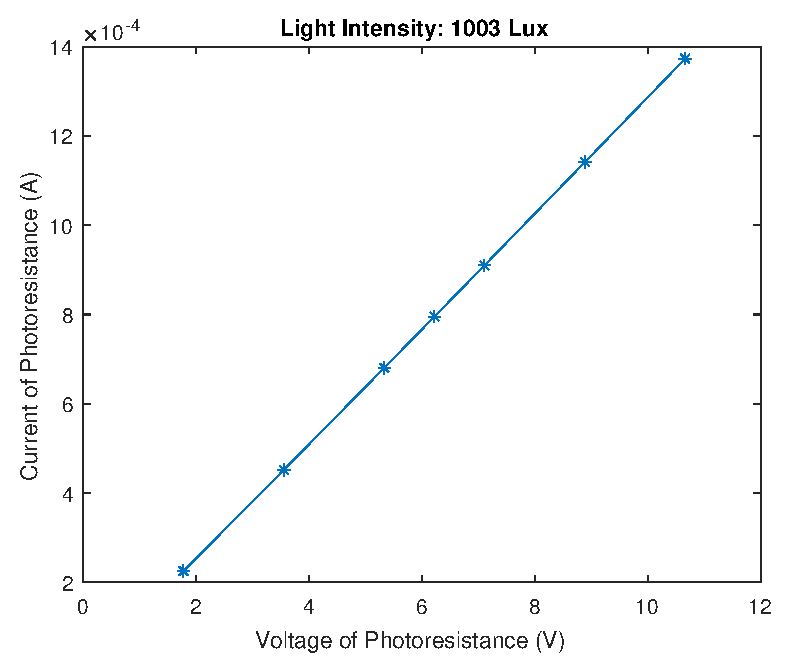
\includegraphics[width=\linewidth]{光电传感器综合实验图像/photoresistor_1003Lux}
    \caption{光照度1003Lux}
  \end{subfigure}
  \begin{subfigure}{.45\textwidth}
    \centering
    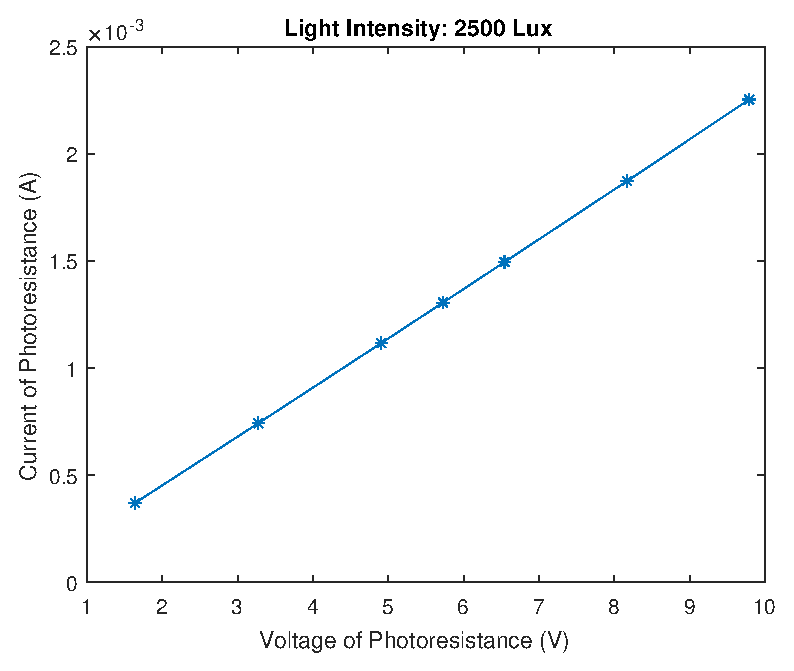
\includegraphics[width=\linewidth]{光电传感器综合实验图像/photoresistor_2500Lux}
    \caption{光照度2500Lux}
  \end{subfigure}
  \begin{subfigure}{.45\textwidth}
    \centering
    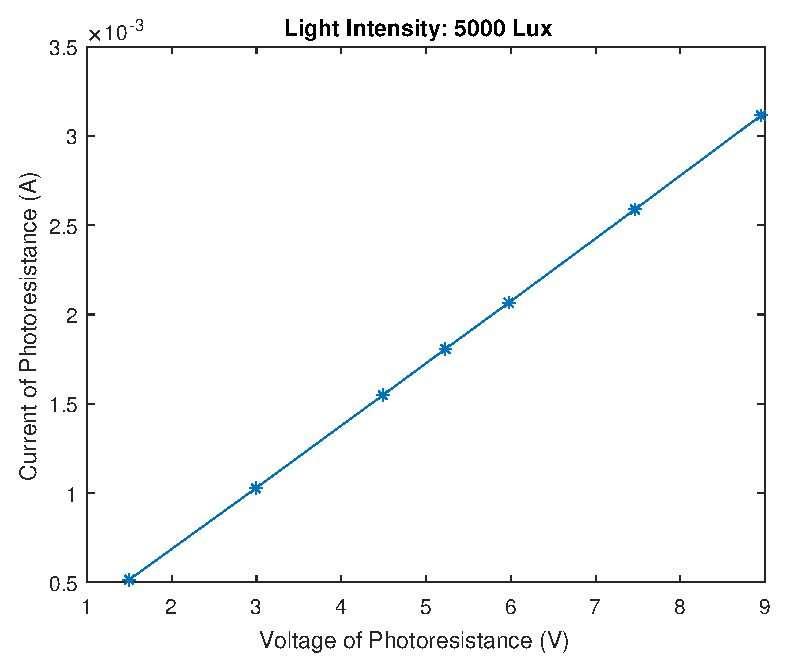
\includegraphics[width=\linewidth]{光电传感器综合实验图像/photoresistor_5000Lux}
    \caption{光照度5000Lux}
  \end{subfigure}
  \begin{subfigure}{.45\textwidth}
    \centering
    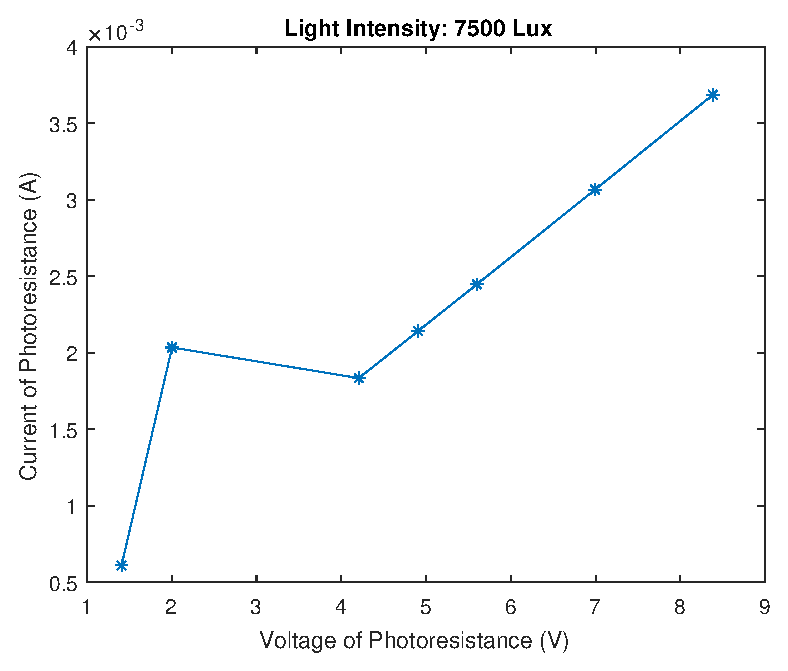
\includegraphics[width=\linewidth]{光电传感器综合实验图像/photoresistor_7500Lux}
    \caption{光照度7500Lux}
  \end{subfigure}
  \caption{光敏电阻伏安特性测量}
\end{figure}

\newpage
\subsubsection{光敏电阻的光照特性测量}

测量时串联的电阻为$981.3\Omega$

\begin{table}[H]
  \centering
  \begin{tabular}{|c|c|c|c|c|c|c|}
    \hline
    光照强度(Lux) &509&1002&1501&2000&2500&3000\\\hline
    电源电压(V) &2.160&2.253&2.324&2.386&2.448&2.499\\\hline
    电阻两端电压(V) &1.5823&0.2488&0.3224&0.3866&0.4450&0.4970\\\hline
    光敏电阻阻值($k\Omega$) & 1.2403&7.8883&6.0875&5.0766&4.4103&3.9489 \\\hline
  \end{tabular}
  \caption{光敏电阻光照特性测量:光敏电阻两端电压2V}
\end{table}

\begin{table}[H]
  \centering
  \begin{tabular}{|c|c|c|c|c|c|c|}
    \hline
    光照强度(Lux) &509&997&1503&2000&2500&3000\\\hline
    电源电压(V) &4.316&4.499&4.652&4.775&4.887&4.999\\\hline
    电阻两端电压(V) &0.3173&0.4965&0.6474&0.7768&0.8900&0.9963\\\hline
    光敏电阻阻值($10 k\Omega$) & 1.2371&0.7906&0.6063&0.5053&0.4410&0.3940\\\hline
  \end{tabular}
  \caption{光敏电阻光照特性测量:光敏电阻两端电压4V}
\end{table}

\begin{table}[H]
  \centering
  \begin{tabular}{|c|c|c|c|c|c|c|}
    \hline
    光照强度(Lux) &509&1007&1498&2000&2500&3000\\\hline
    电源电压(V) &6.476&6.752&6.973&7.166&7.338&7.502\\\hline
    电阻两端电压(V) &0.4786&0.7531&0.9734&1.1696&1.3401&1.5013\\\hline
    光敏电阻阻值($10k\Omega$) & 1.2302&0.7818&0.6049&0.5034&0.4394&0.3922\\\hline
  \end{tabular}
  \caption{光敏电阻光照特性测量:光敏电阻两端电压6V}
\end{table}

\begin{table}[H]
  \centering
  \begin{tabular}{|c|c|c|c|c|c|c|}
    \hline
    光照强度(Lux) &504&1001&1501&2000&2500&3000\\\hline
    电源电压(V) &8.625&8.999&9.303&9.559&9.801&10.011\\\hline
    电阻两端电压(V) &0.6342&1.0016&1.3004&1.5637&1.7975&2.0095\\\hline
    光敏电阻阻值($10k\Omega$) & 1.2378&0.7838&0.6037&0.5020&0.4367&0.3907\\\hline
  \end{tabular}
  \caption{光敏电阻光照特性测量:光敏电阻两端电压8V}
\end{table}

\begin{table}[H]
  \centering
  \begin{tabular}{|c|c|c|c|c|c|c|}
    \hline
    光照强度(Lux) &504&1001&1499&2000&2500&3000\\\hline
    电源电压(V) &10.804&11.256&11.627&11.956&12.254&12.510\\\hline
    电阻两端电压(V) &0.7987&1.2554&1.6288&1.9584&2.2483&2.5132\\\hline
    光敏电阻阻值($10k\Omega$) & 1.2286&0.7817&0.6025&0.5011&0.4365&0.3905\\\hline
  \end{tabular}
  \caption{光敏电阻光照特性测量:光敏电阻两端电压10V}
\end{table}

\begin{figure}[H]
  \centering
  \begin{subfigure}{.45\textwidth}
    \centering
    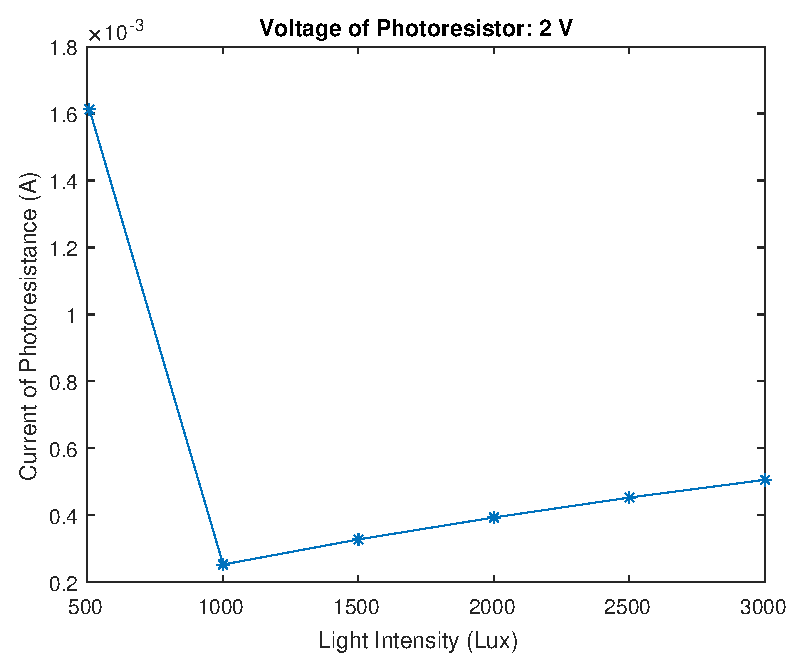
\includegraphics[width=\linewidth]{光电传感器综合实验图像/photoresistor_2V}
  \caption{光敏电阻两端电压2V}
  \end{subfigure}
  \begin{subfigure}{.45\textwidth}
    \centering
    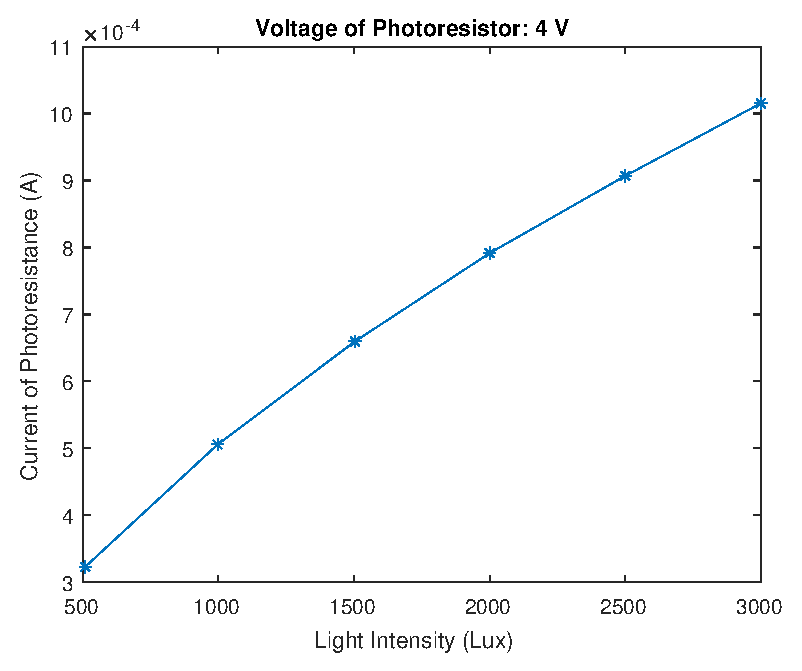
\includegraphics[width=\linewidth]{光电传感器综合实验图像/photoresistor_4V}
  \caption{光敏电阻两端电压4V}
  \end{subfigure}
  \begin{subfigure}{.45\textwidth}
    \centering
    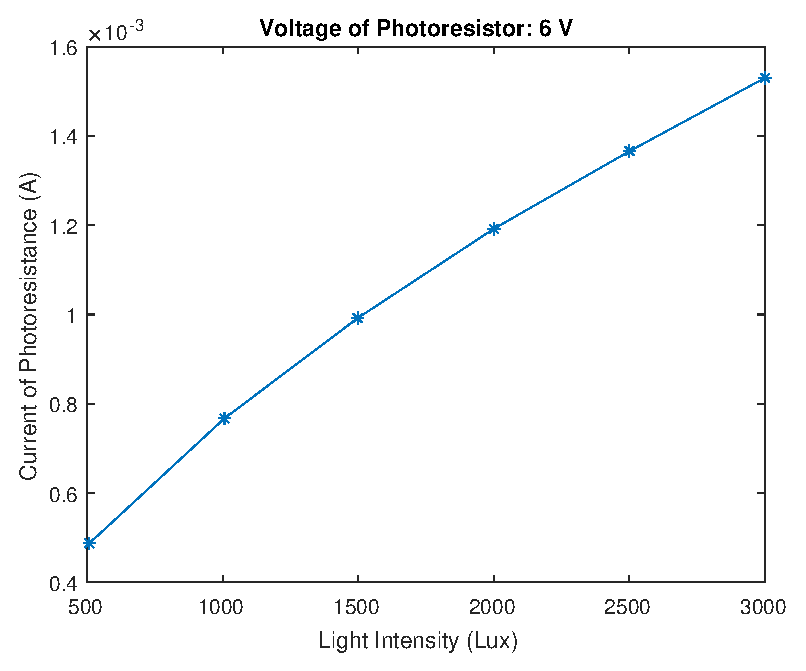
\includegraphics[width=\linewidth]{光电传感器综合实验图像/photoresistor_6V}
  \caption{光敏电阻两端电压6V}
  \end{subfigure}
  \begin{subfigure}{.45\textwidth}
    \centering
    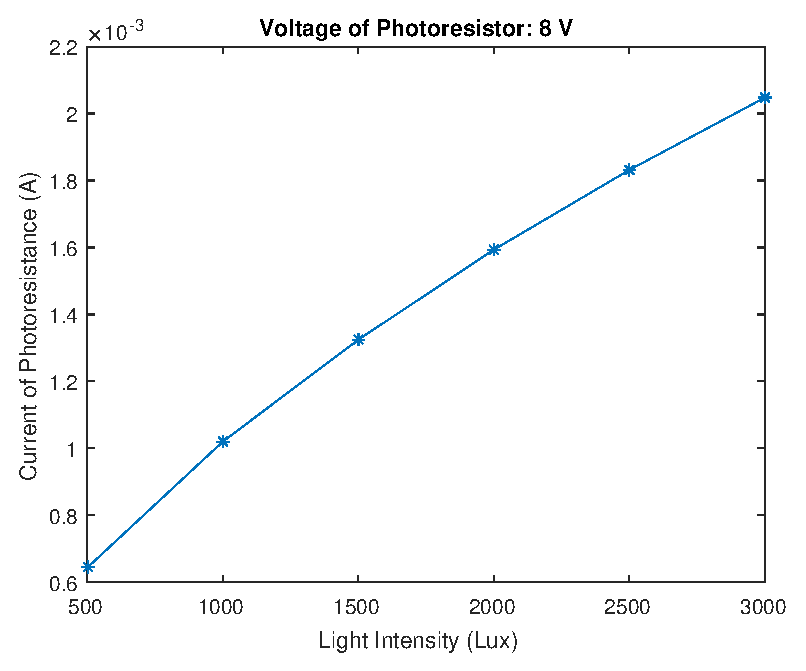
\includegraphics[width=\linewidth]{光电传感器综合实验图像/photoresistor_8V}
  \caption{光敏电阻两端电压8V}
  \end{subfigure}
  \begin{subfigure}{.45\textwidth}
    \centering
    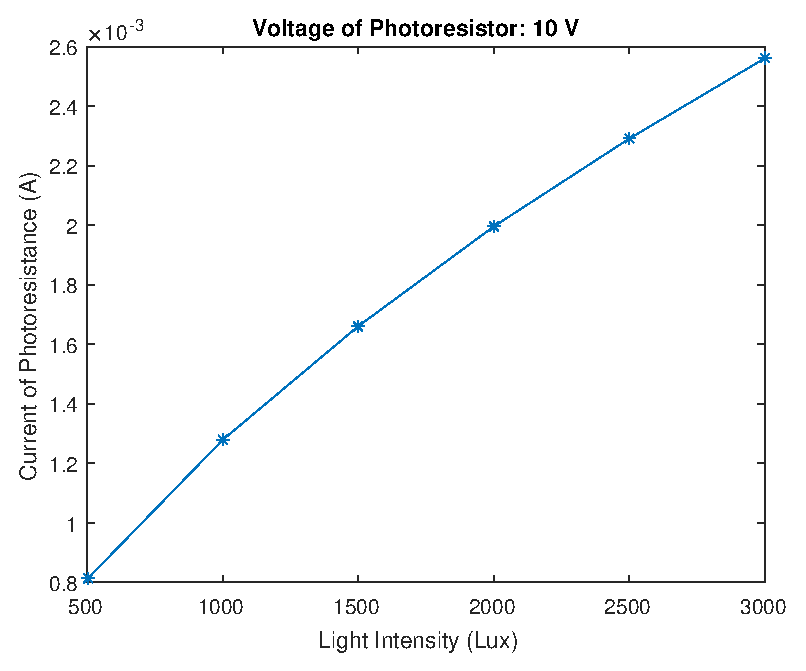
\includegraphics[width=\linewidth]{光电传感器综合实验图像/photoresistor_10V}
  \caption{光敏电阻两端电压10V}
  \end{subfigure}
  \caption{光敏电阻光照特性测量}
\end{figure}

\newpage
\subsubsection{硅光电池的伏安特性测量}

测量时取样电阻为$100\Omega$

\begin{table}[H]
  \centering
  \begin{tabular}{|c|c|c|c|c|c|c|c|}
    \hline
    负载电阻(欧姆) &无穷&0&1000&2000&5100&7500&10000\\\hline
    光电压(mV) &329.4&1.06&10.50&20.27&49.73&72.16&96.63\\\hline
  \end{tabular}
  \caption{硅光电池伏安特性测量:光照度503Lux}
\end{table}

\begin{table}[H]
  \centering
  \begin{tabular}{|c|c|c|c|c|c|c|c|}
    \hline
    负载电阻(欧姆) &无穷&0&1000&2000&5100&7500&10000\\\hline
    光电压(mV) &362.5&1.89&20.38&39.32&96.03&138.18&181.21\\\hline
  \end{tabular}
  \caption{硅光电池伏安特性测量:光照度1003Lux}
\end{table}

\begin{table}[H]
  \centering
  \begin{tabular}{|c|c|c|c|c|c|c|c|}
    \hline
    负载电阻(欧姆) &无穷&0&1000&2000&5100&7500&10000\\\hline
    光电压(mV) &379.9&2.84&30.56&58.97&143.3&201.99&253.54\\\hline
  \end{tabular}
  \caption{硅光电池伏安特性测量:光照度1495Lux}
\end{table}

\begin{table}[H]
  \centering
  \begin{tabular}{|c|c|c|c|c|c|c|c|}
    \hline
    负载电阻(欧姆) &无穷&0&1000&2000&5100&7500&10000\\\hline
    光电压(mV) &391.7&3.79&41.07&79.26&189.56&257.23&304.8\\\hline
  \end{tabular}
  \caption{硅光电池伏安特性测量:光照度2000Lux}
\end{table}

\begin{table}[H]
  \centering
  \begin{tabular}{|c|c|c|c|c|c|c|c|}
    \hline
    负载电阻(欧姆) &无穷&0&1000&2000&5100&7500&10000\\\hline
    光电压(mV) &400.1&4.74&51.35&99.03&231.20&298.90&336.0\\\hline
  \end{tabular}
  \caption{硅光电池伏安特性测量:光照度2500Lux}
\end{table}

\begin{table}[H]
  \centering
  \begin{tabular}{|c|c|c|c|c|c|c|c|}
    \hline
    负载电阻(欧姆) &无穷&0&1000&2000&5100&7500&10000\\\hline
    光电压(mV) &406.10&5.81&61.53&118.16&267.14&327.60&355.5\\\hline
  \end{tabular}
  \caption{硅光电池伏安特性测量:光照度3000Lux}
\end{table}

\begin{figure}[H]
  \centering
  \begin{subfigure}{.45\textwidth}
    \centering
    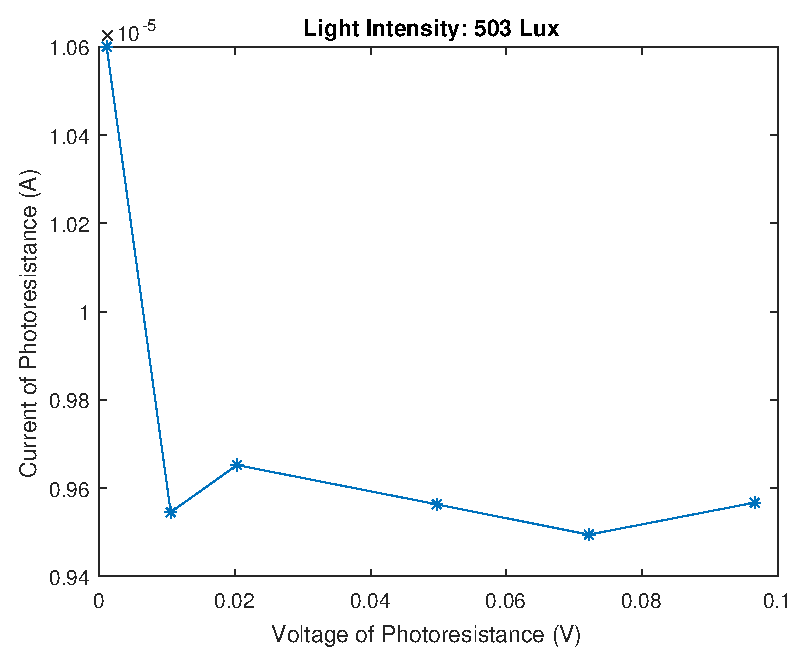
\includegraphics[width=\linewidth]{光电传感器综合实验图像/photocell_503Lux}
    \caption{光照度503Lux}
  \end{subfigure}
  \begin{subfigure}{.45\textwidth}
    \centering
    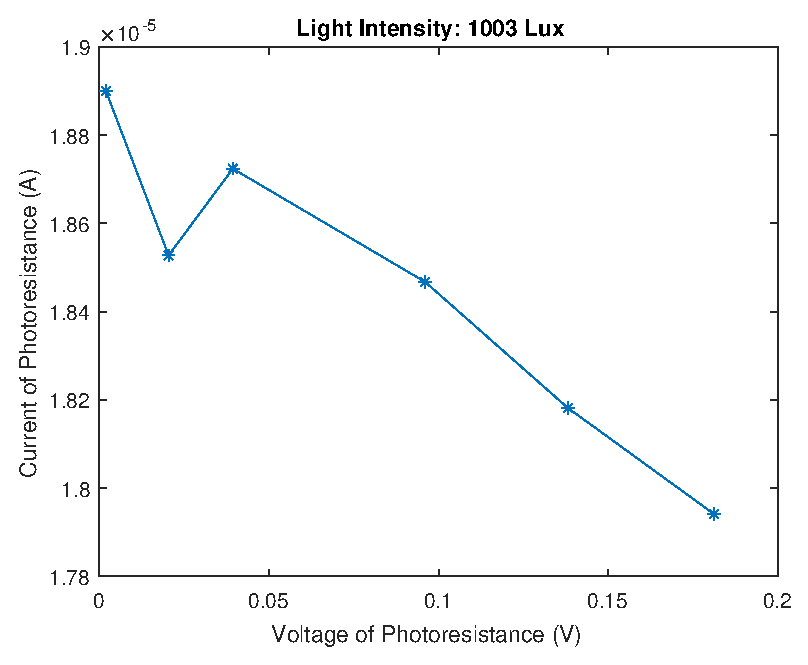
\includegraphics[width=\linewidth]{光电传感器综合实验图像/photocell_1003Lux}
    \caption{光照度1003Lux}
  \end{subfigure}
  \begin{subfigure}{.45\textwidth}
    \centering
    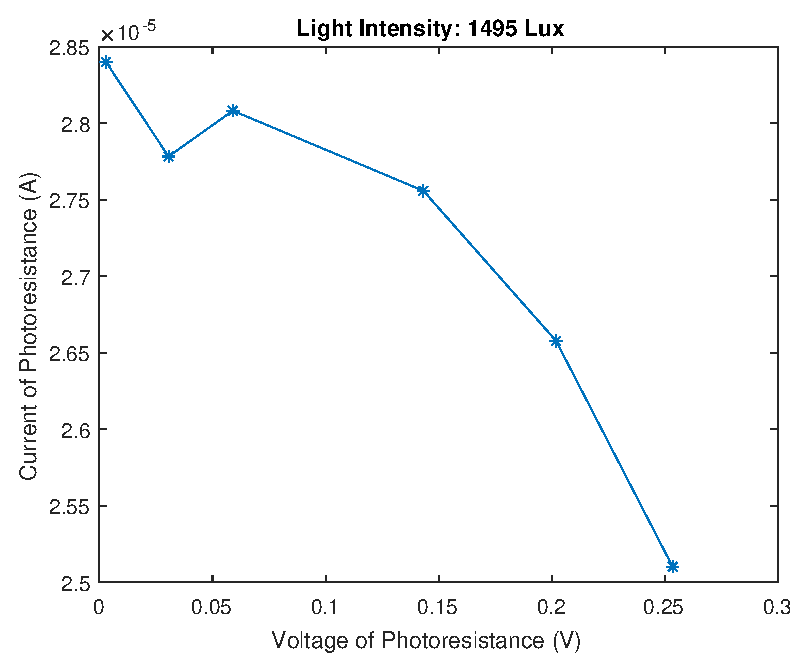
\includegraphics[width=\linewidth]{光电传感器综合实验图像/photocell_1495Lux}
    \caption{光照度1495Lux}
  \end{subfigure}
  \begin{subfigure}{.45\textwidth}
    \centering
    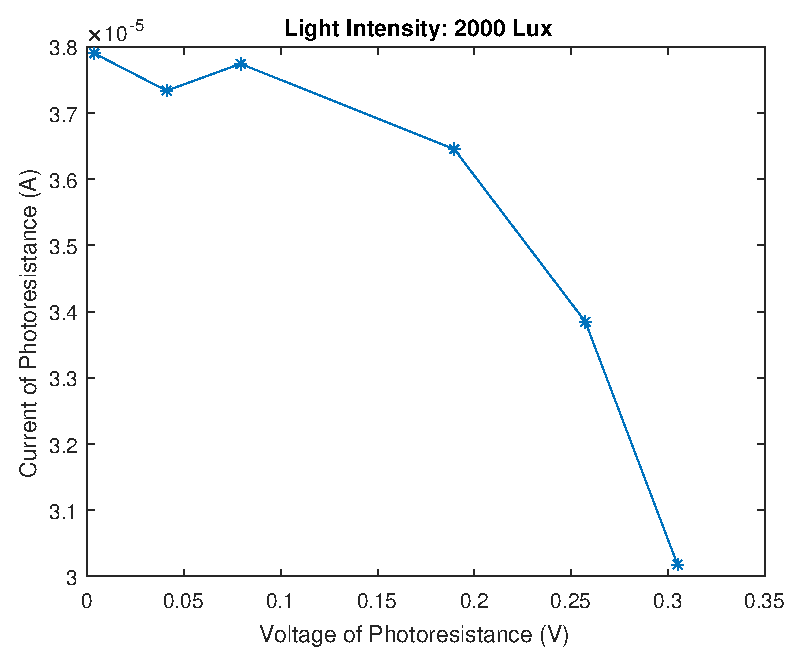
\includegraphics[width=\linewidth]{光电传感器综合实验图像/photocell_2000Lux}
    \caption{光照度2000Lux}
  \end{subfigure}
  \begin{subfigure}{.45\textwidth}
    \centering
    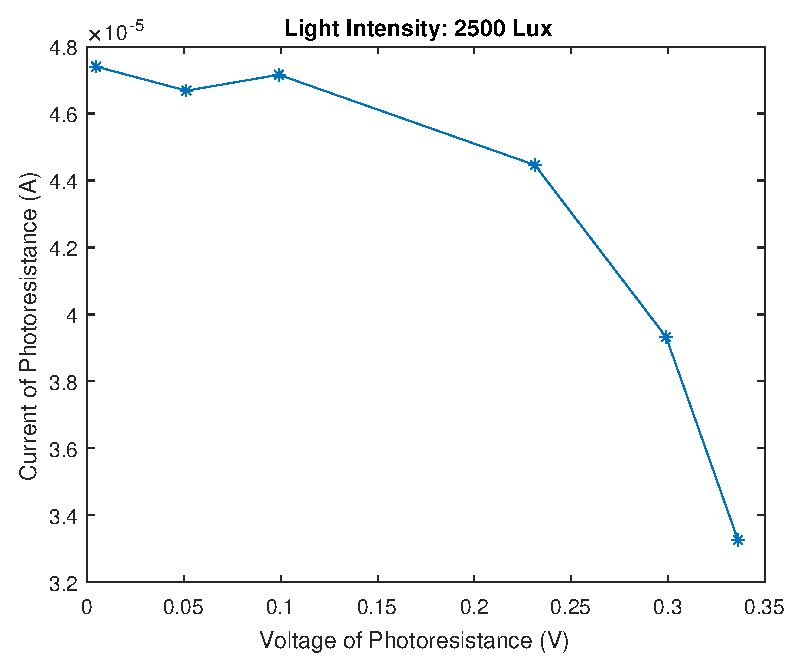
\includegraphics[width=\linewidth]{光电传感器综合实验图像/photocell_2500Lux}
    \caption{光照度2500Lux}
  \end{subfigure}
  \begin{subfigure}{.45\textwidth}
    \centering
    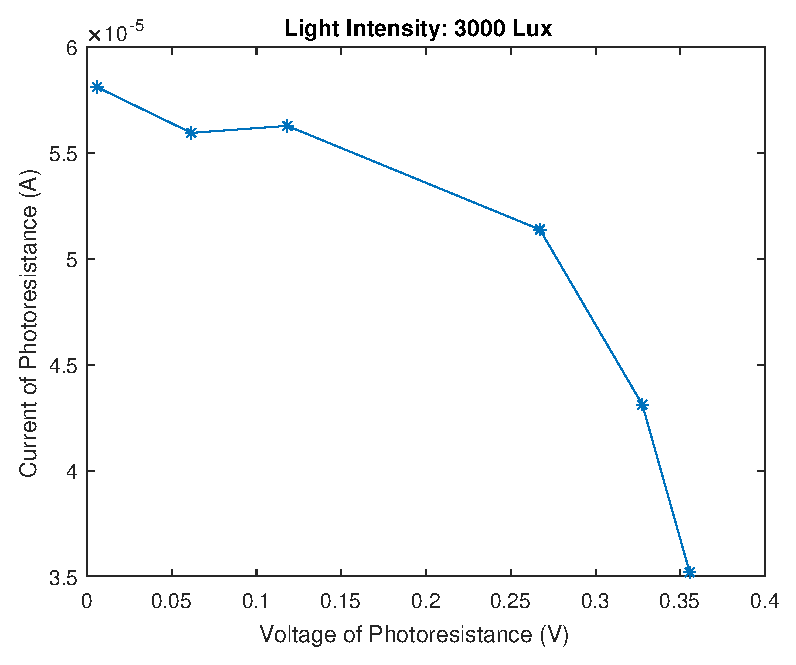
\includegraphics[width=\linewidth]{光电传感器综合实验图像/photocell_3000Lux}
    \caption{光照度3000Lux}
  \end{subfigure}
  \caption{硅光电池伏安特性测量}
\end{figure}

\subsubsection{硅光电池的光照特性测量}

\begin{table}[H]
  \centering
  \begin{tabular}{|c|c|c|c|c|c|c|c|}
    \hline
    光照强度(Lux) &503&1003&1495&2000&2500&3000\\\hline
    短路电流($10^{-2}$mA) &1.06&1.89&2.84&3.79&4.74&5.81\\\hline
    开路电压(mV) &329.4&362.5&379.9&391.7&400.1&406.10\\\hline
  \end{tabular}
  \caption{硅光电池光照特性测量}
\end{table}

\subsubsection{光电二极管的伏安特性测量}

测量时串联的电阻为$1.002M\Omega$

\begin{table}[H]
  \centering
  \begin{tabular}{|c|c|c|c|c|c|c|c|}
    \hline
    电源电压(V) &0.6561&1.0113&2.0054&4.167&6.533&9.025&12.322\\\hline
    电阻两端电压(mV) &135.23&135.81&137.00&138.14&138.85&140.000&140.30\\\hline
    光电二极管电阻($10M\Omega$) & 0.3859&0.6459&1.3665&2.9223&4.6143&6.3591&8.7000\\\hline
  \end{tabular}
  \caption{光电二极管伏安特性测量:光照强度506Lux}
\end{table}

\begin{table}[H]
  \centering
  \begin{tabular}{|c|c|c|c|c|c|c|c|}
    \hline
    电源电压(V) &0.6044&1.0094&2.011&4.127&6.554&9.273&12.325\\\hline
    电阻两端电压(mV) &244.45&265.03&268.52&270.53&271.90&273.30&274.58\\\hline
    光电二极管电阻($10M\Omega$) & 0.1475&0.2814&0.6502&1.4284&2.3151&3.2996&4.3975\\\hline
  \end{tabular}
  \caption{光电二极管伏安特性测量:光照强度1008Lux}
\end{table}

\begin{table}[H]
  \centering
  \begin{tabular}{|c|c|c|c|c|c|c|c|}
    \hline
    电源电压(V) &0.6558&1.0215&2.093&4.117&6.552&9.219&12.312\\\hline
    电阻两端电压(V) &0.5319&0.5403&0.5460&0.5507&0.5532&0.5562&0.5587\\\hline
    光电二极管电阻($10M\Omega$) & 0.0233&0.0892&0.2839&0.6489&1.0866&1.5606&2.1079\\\hline
  \end{tabular}
  \caption{光电二极管伏安特性测量:光照强度2000Lux}
\end{table}

\begin{table}[H]
  \centering
  \begin{tabular}{|c|c|c|c|c|c|c|c|}
    \hline
    电源电压(V) &0.8612&1.0227&2.032&4.124&6.534&9.201&12.314\\\hline
    电阻两端电压(V) &0.7940&0.7965&0.8048&0.8120&0.8166&0.8204&0.8240\\\hline
    光电二极管电阻($10M\Omega$) & 0.0085&0.0285&0.1528&0.4087&0.7015&1.0236&1.3972\\\hline
  \end{tabular}
  \caption{光电二极管伏安特性测量:光照强度3000Lux}
\end{table}

\begin{figure}[H]
  \centering
  \begin{subfigure}{.45\textwidth}
    \centering
    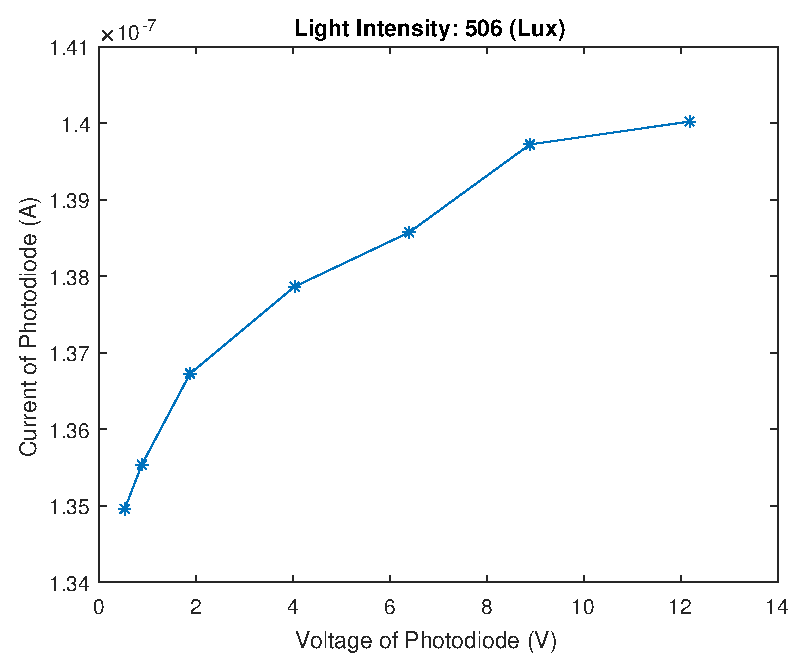
\includegraphics[width=\linewidth]{光电传感器综合实验图像/photodiode_506Lux}
    \caption{光照强度506Lux}
  \end{subfigure}
  \begin{subfigure}{.45\textwidth}
    \centering
    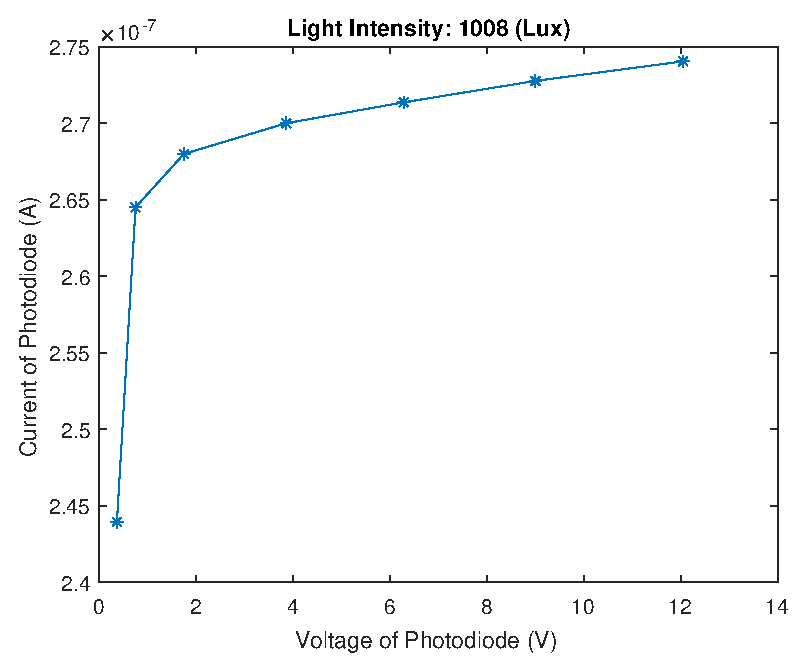
\includegraphics[width=\linewidth]{光电传感器综合实验图像/photodiode_1008Lux}
    \caption{光照强度1008Lux}
  \end{subfigure}
  \begin{subfigure}{.45\textwidth}
    \centering
    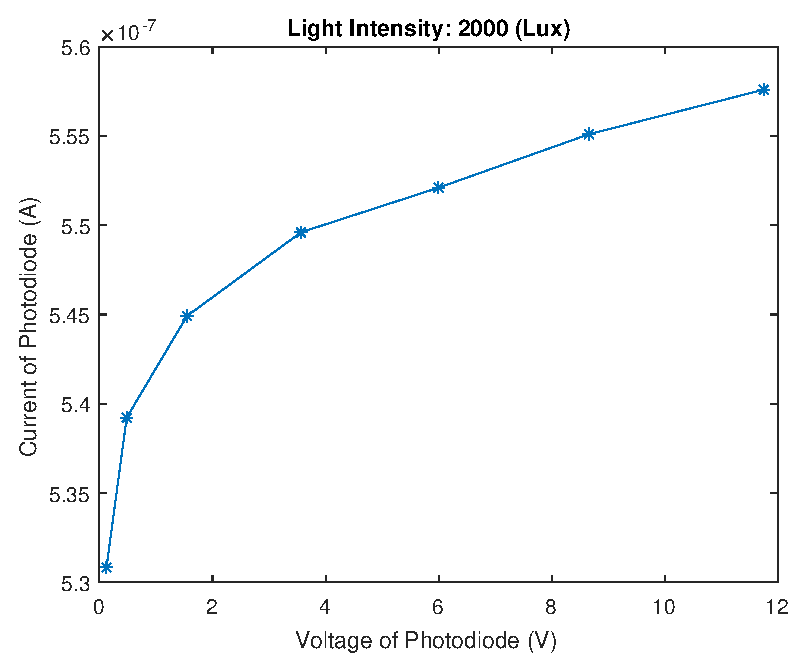
\includegraphics[width=\linewidth]{光电传感器综合实验图像/photodiode_2000Lux}
    \caption{光照强度2000Lux}
  \end{subfigure}
  \begin{subfigure}{.45\textwidth}
    \centering
    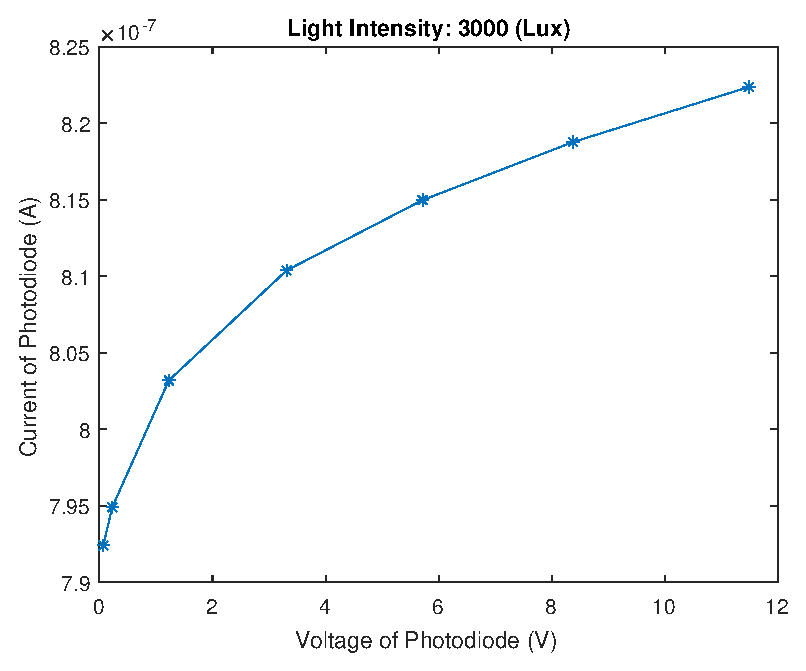
\includegraphics[width=\linewidth]{光电传感器综合实验图像/photodiode_3000Lux}
    \caption{光照强度3000Lux}
  \end{subfigure}
  \caption{光电二极管伏安特性测量}
\end{figure}

\newpage
\subsubsection{光电二极管的光照特性测量}

测量时串联的电阻为$1.002M\Omega$

\begin{table}[H]
  \centering
  \begin{tabular}{|c|c|c|c|c|c|c|}
    \hline
    光照强度(Lux) &504&1008&1503&2000&2500&3000\\\hline
    电源电压(V) &2.136&2.271&2.405&2.540&2.674&2.800\\\hline
    电阻两端电压(V) &0.137&0.271&0.405&0.540&0.674&0.804\\\hline
    光电二极管电阻($10M\Omega$) & 1.4628&0.7395&0.4948&0.3711&0.2973&0.2493\\\hline
  \end{tabular}
  \caption{光电二极管光照特性测量:光电二极管两端电压2V}
\end{table}

\begin{table}[H]
  \centering
  \begin{tabular}{|c|c|c|c|c|c|c|}
    \hline
    光照强度(Lux) &497&1008&1498&2000&2500&3000\\\hline
    电源电压(V) &4.138&4.274&4.406&4.544&4.684&4.807\\\hline
    电阻两端电压(V) &0.135&0.272&0.405&0.541&0.677&0.809\\\hline
    光电二极管电阻($10M\Omega$) & 2.9689&1.4735&0.9896&0.7409&0.5920&0.4954\\\hline
  \end{tabular}
  \caption{光电二极管光照特性测量:光电二极管两端电压4V}
\end{table}

\begin{table}[H]
  \centering
  \begin{tabular}{|c|c|c|c|c|c|c|}
    \hline
    光照强度(Lux) &497&1005&1499&2000&2500&3000\\\hline
    电源电压(V) &6.138&6.264&6.409&6.537&6.679&6.811\\\hline
    电阻两端电压(V) &0.135&0.273&0.4062&0.5440&0.6774&0.8110\\\hline
    光电二极管电阻($10M\Omega$) & 4.4533&2.2022&1.4801&1.1051&0.8875&0.7413\\\hline
  \end{tabular}
  \caption{光电二极管光照特性测量:光电二极管两端电压6V}
\end{table}

\begin{table}[H]
  \centering
  \begin{tabular}{|c|c|c|c|c|c|c|}
    \hline
    光照强度(Lux) &504&1000&1503&2000&2500&3000\\\hline
    电源电压(V) &8.143&8.277&8.410&8.554&8.677&8.811\\\hline
    电阻两端电压(V) &0.138&0.271&0.4088&0.5474&0.6804&0.8136\\\hline
    光电二极管电阻($10M\Omega$) & 5.8087&2.9579&1.9609&1.4644&1.1781&0.9853\\\hline
  \end{tabular}
  \caption{光电二极管光照特性测量:光电二极管两端电压8V}
\end{table}

\begin{figure}[H]
  \centering
  \begin{subfigure}{.45\textwidth}
    \centering
    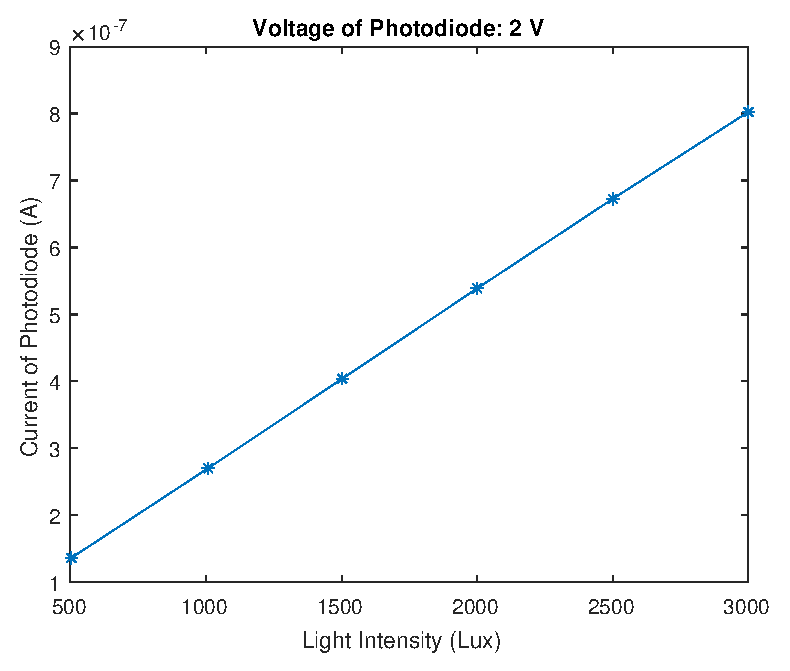
\includegraphics[width=\linewidth]{光电传感器综合实验图像/photodiode_2V}
    \caption{光电二极管两端电压2V}
  \end{subfigure}
  \begin{subfigure}{.45\textwidth}
    \centering
    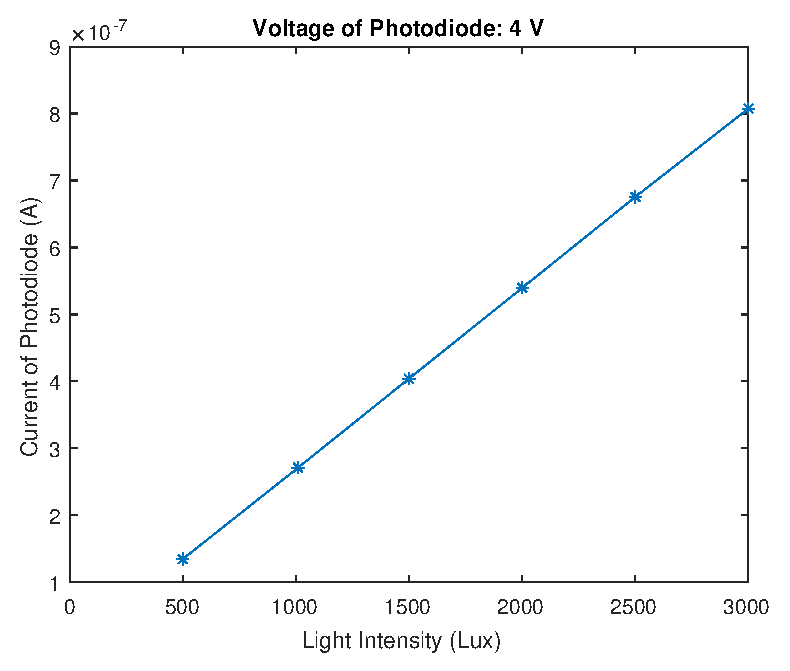
\includegraphics[width=\linewidth]{光电传感器综合实验图像/photodiode_4V}
    \caption{光电二极管两端电压4V}
  \end{subfigure}
  \begin{subfigure}{.45\textwidth}
    \centering
    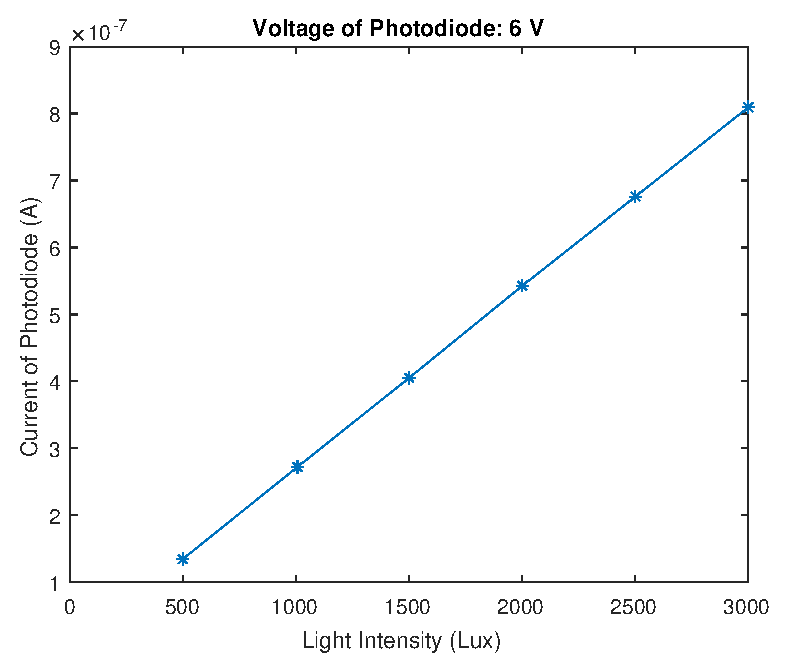
\includegraphics[width=\linewidth]{光电传感器综合实验图像/photodiode_6V}
    \caption{光电二极管两端电压6V}
  \end{subfigure}
  \begin{subfigure}{.45\textwidth}
    \centering
    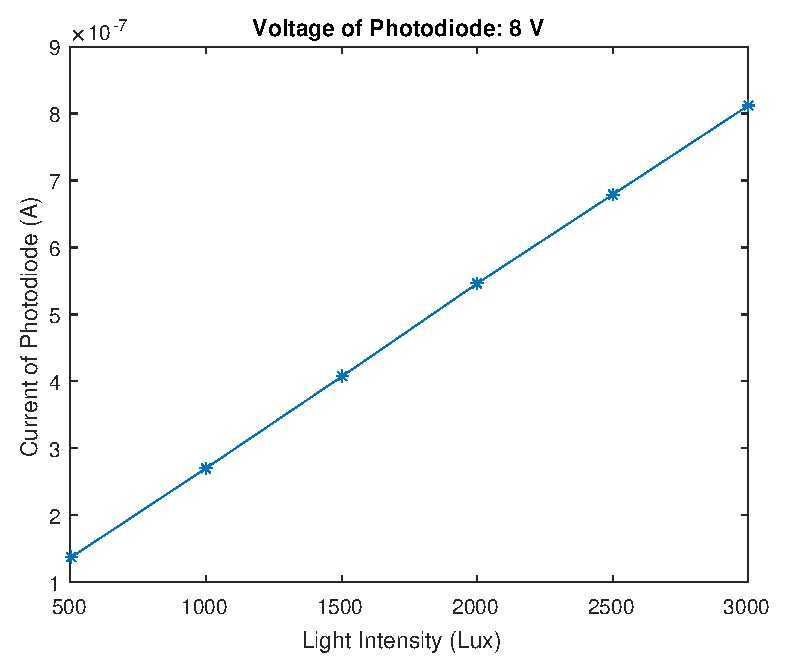
\includegraphics[width=\linewidth]{光电传感器综合实验图像/photodiode_8V}
    \caption{光电二极管两端电压8V}
  \end{subfigure}
  \caption{光电二极管光照特性测量}
\end{figure}

\newpage
\subsubsection{光电三极管的伏安特性测量}

测量时串联的电阻为$203.32k\Omega$

\begin{table}[H]
  \centering
  \begin{tabular}{|c|c|c|c|c|c|c|c|}
    \hline
    电源电压(V) &1.02&3.020&5.04&7.01&9.00&15.13&17.4\\\hline
    电阻两端电压(mV) &0.07&0.09&0.11&0.14&0.22&5.64&7.83\\\hline
    光电三极管电阻($M\Omega$) &2.7593&6.6192&9.1124&9.9772&8.1143&0.3421&0.2485 \\\hline
  \end{tabular}
  \caption{光电三极管伏安特性测量:光照强度517Lux}
\end{table}

\begin{table}[H]
  \centering
  \begin{tabular}{|c|c|c|c|c|c|c|c|}
    \hline
    电源电压(V) &1.01&3.03&5.05&7.06&12.8&15.08&17.06\\\hline
    电阻两端电压(mV) &0.13&0.16&0.20&0.26&2.61&5.58&7.55\\\hline
    光电三极管电阻($M\Omega$) & 1.3763&3.6471&4.9305&5.3176&0.7938&0.3462&0.2561\\\hline
  \end{tabular}
  \caption{光电三极管伏安特性测量:光照强度1002Lux}
\end{table}

\begin{table}[H]
  \centering
  \begin{tabular}{|c|c|c|c|c|c|c|c|}
    \hline
    电源电压(V) &1.04&3.50&6.02&8.52&10.06&11.05&13.00\\\hline
    电阻两端电压(V) &0.19&0.25&0.34&0.51&1.17&1.54&3.53\\\hline
    光电三极管电阻($M\Omega$) &0.9096&2.6432&3.3966&3.1933&1.5449&1.2556&0.5455 \\\hline
  \end{tabular}
  \caption{光电三极管伏安特性测量:光照强度1505Lux}
\end{table}

\begin{table}[H]
  \centering
  \begin{tabular}{|c|c|c|c|c|c|c|c|}
    \hline
    电源电压(V) &1.05&3.03&5.01&7.04&9.03&11.01&13.06\\\hline
    电阻两端电压(V) &0.05&0.07&0.08&0.12&0.19&1.58&3.59\\\hline
    光电三极管电阻($M\Omega$) & 4.066&8.598&12.530&11.725&9.460&1.213&0.536\\\hline
  \end{tabular}
  \caption{光电三极管伏安特性测量:光照强度2000Lux}
\end{table}

\begin{figure}[H]
  \centering
  \begin{subfigure}{.45\textwidth}
    \centering
    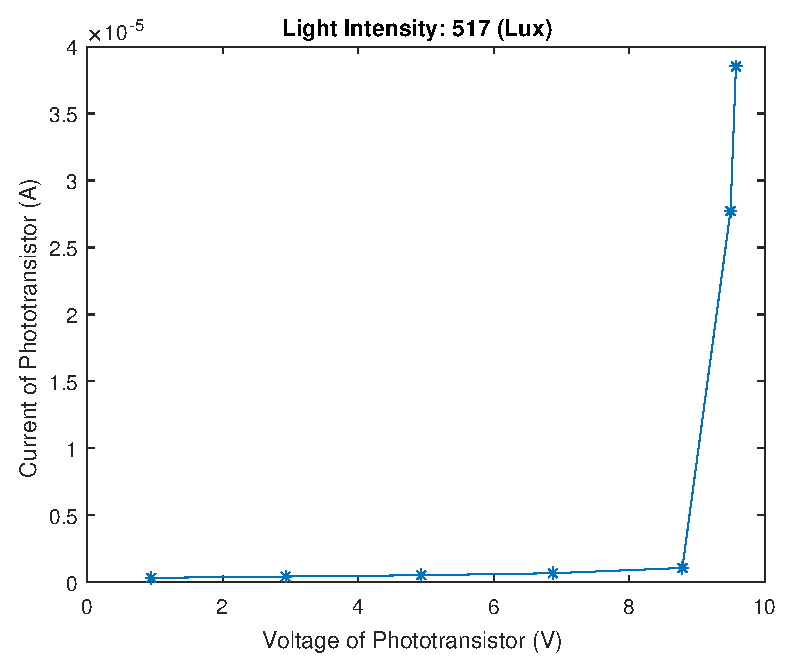
\includegraphics[width=\linewidth]{光电传感器综合实验图像/phototransistor_517Lux}
    \caption{光照强度517Lux}
  \end{subfigure}
  \begin{subfigure}{.45\textwidth}
    \centering
    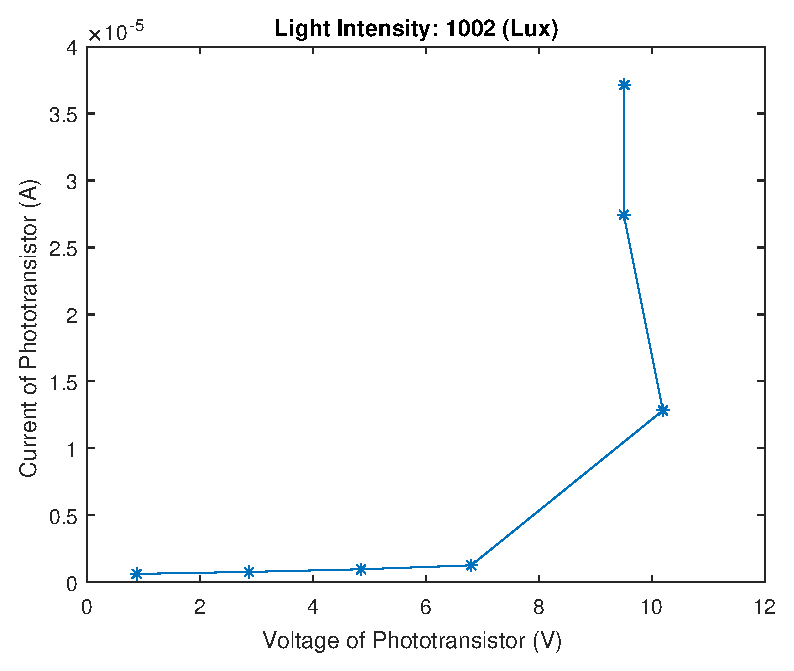
\includegraphics[width=\linewidth]{光电传感器综合实验图像/phototransistor_1002Lux}
    \caption{光照强度1002Lux}
  \end{subfigure}
  \begin{subfigure}{.45\textwidth}
    \centering
    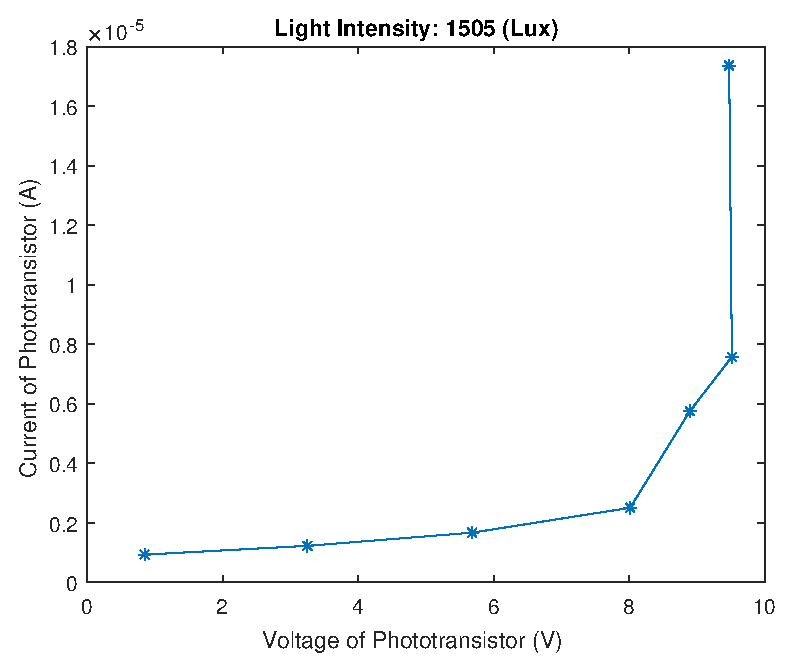
\includegraphics[width=\linewidth]{光电传感器综合实验图像/phototransistor_1505Lux}
    \caption{光照强度1505Lux}
  \end{subfigure}
  \begin{subfigure}{.45\textwidth}
    \centering
    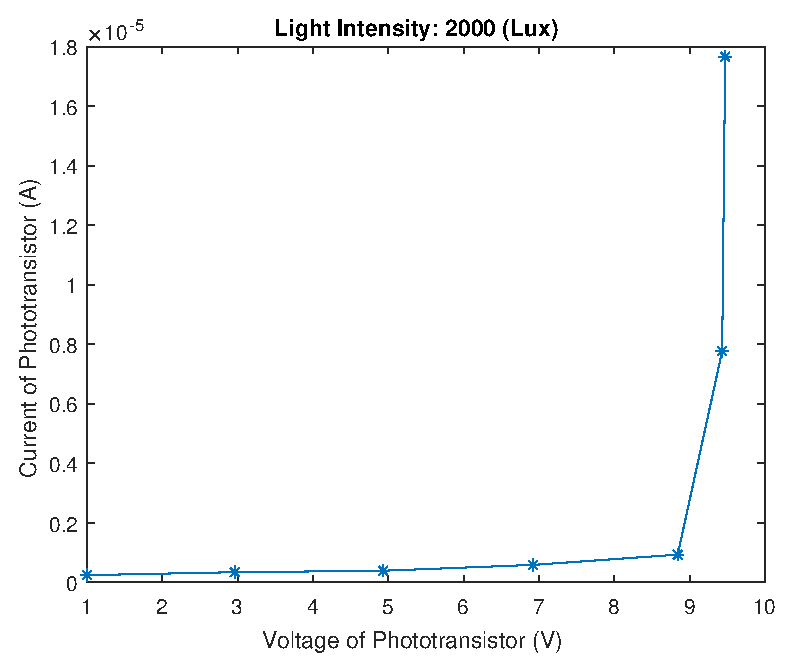
\includegraphics[width=\linewidth]{光电传感器综合实验图像/phototransistor_2000Lux}
    \caption{光照强度2000Lux}
  \end{subfigure}
  \caption{光电三极管伏安特性测量}
\end{figure}

\newpage
\subsubsection{光电三极管的光照特性测量}

测量时串联的电阻为$203.32k\Omega$

\begin{table}[H]
  \centering
  \begin{tabular}{|c|c|c|c|c|c|c|}
    \hline
    光照强度(Lux) &505&1000&1505&2000&2500&3000\\\hline
    电源电压(V) &2.02&2.03&2.04&2.06&2.07&2.09\\\hline
    电阻两端电压(V) &0.02&0.03&0.04&0.06&0.07&0.09\\\hline
    光电三极管电阻($10M\Omega$) &2.0332&1.3555&1.0166&0.6777&0.5809&0.4518 \\\hline
  \end{tabular}
  \caption{光电三极管光照特性测量:光电三极管两端电压2V}
\end{table}

\begin{table}[H]
  \centering
  \begin{tabular}{|c|c|c|c|c|c|c|}
    \hline
    光照强度(Lux) &506&1005&1508&2000&2500&3000\\\hline
    电源电压(V) &4.02&4.04&4.06&4.08&4.10&4.11\\\hline
    电阻两端电压(V) &0.02&0.04&0.06&0.08&0.10&0.11\\\hline
    光电三极管电阻($10M\Omega$) &4.0664&2.0332&1.3555&1.0166&0.8133&0.7393 \\\hline
  \end{tabular}
  \caption{光电三极管光照特性测量:光电三极管两端电压4V}
\end{table}

\begin{table}[H]
  \centering
  \begin{tabular}{|c|c|c|c|c|c|c|}
    \hline
    光照强度(Lux) &506&1002&1498&2000&2500&3000\\\hline
    电源电压(V) &6.03&6.05&6.08&6.10&6.13&6.15\\\hline
    电阻两端电压(V) &0.03&0.05&0.08&0.10&0.13&0.15\\\hline
    光电三极管电阻($10M\Omega$) &4.0664&2.4398&1.5249&1.2199&0.9384&0.8133 \\\hline
  \end{tabular}
  \caption{光电三极管光照特性测量:光电三极管两端电压6V}
\end{table}

\begin{table}[H]
  \centering
  \begin{tabular}{|c|c|c|c|c|c|c|}
    \hline
    光照强度(Lux) &509&1001&1508&2000&2500&3000\\\hline
    电源电压(V) &8.04&8.07&8.11&8.15&8.19&8.22\\\hline
    电阻两端电压(V) &0.04&0.07&0.11&0.15&0.19&0.22\\\hline
    光电三极管电阻($10M\Omega$) &4.0664&2.3237&1.4787&1.0844&0.8561&0.7393 \\\hline
  \end{tabular}
  \caption{光电三极管光照特性测量:光电三极管两端电压8V}
\end{table}

\begin{figure}[H]
  \centering
  \begin{subfigure}{.45\textwidth}
    \centering
    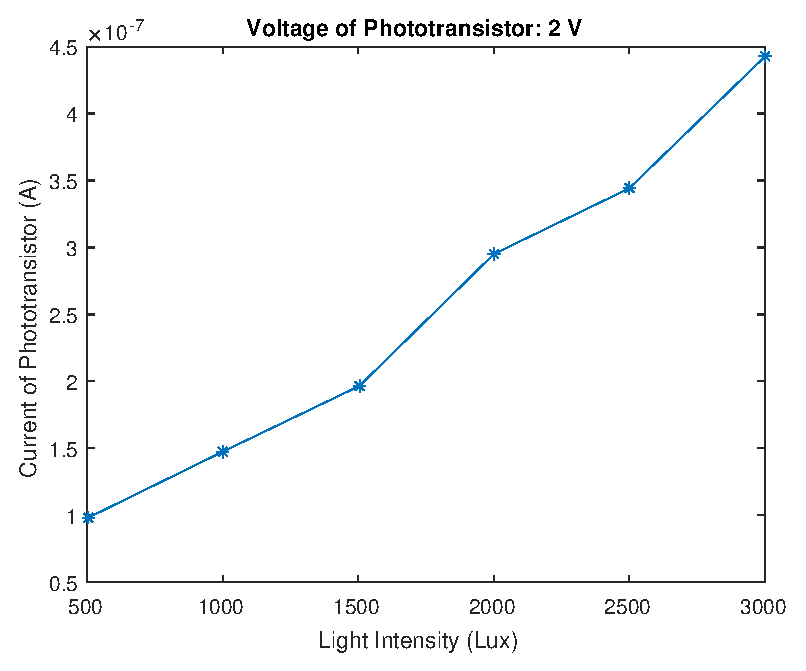
\includegraphics[width=\linewidth]{光电传感器综合实验图像/phototransistor_2V}
    \caption{光电三极管两端电压2V}
  \end{subfigure}
  \begin{subfigure}{.45\textwidth}
    \centering
    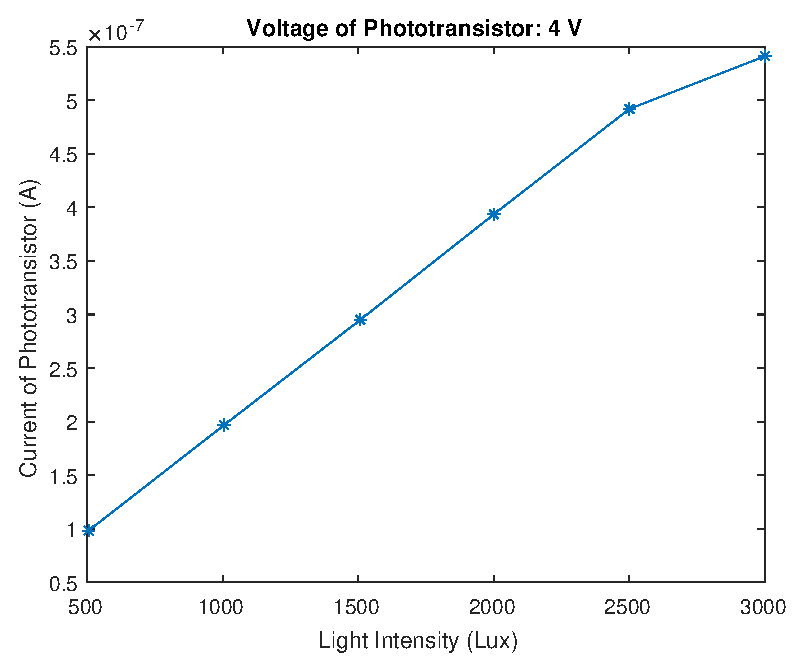
\includegraphics[width=\linewidth]{光电传感器综合实验图像/phototransistor_4V}
    \caption{光电三极管两端电压4V}
  \end{subfigure}
  \begin{subfigure}{.45\textwidth}
    \centering
    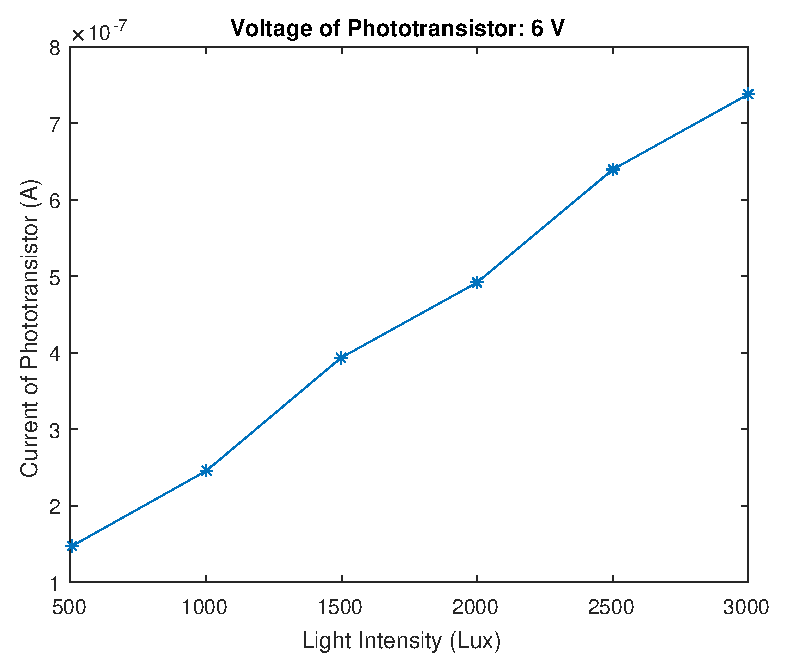
\includegraphics[width=\linewidth]{光电传感器综合实验图像/phototransistor_6V}
    \caption{光电三极管两端电压6V}
  \end{subfigure}
  \begin{subfigure}{.45\textwidth}
    \centering
    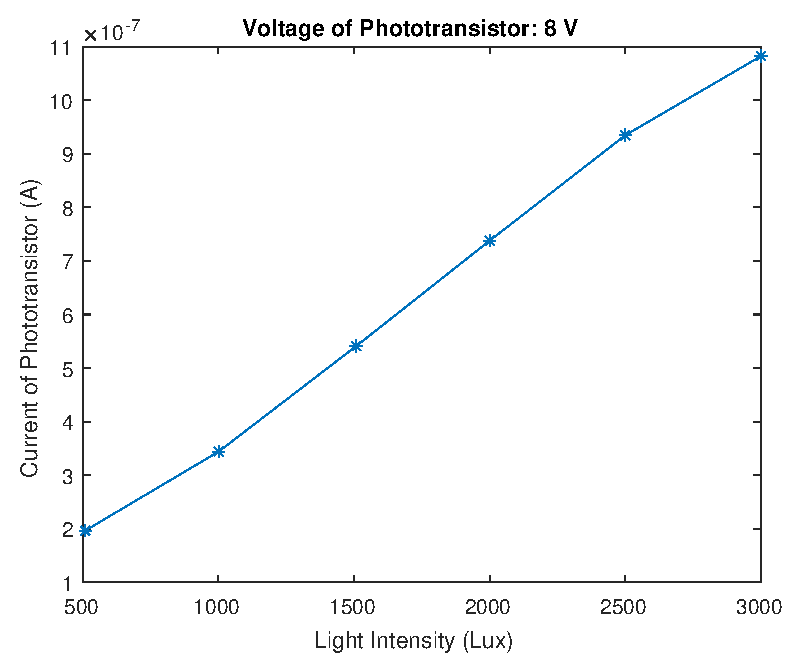
\includegraphics[width=\linewidth]{光电传感器综合实验图像/phototransistor_8V}
    \caption{光电三极管两端电压8V}
  \end{subfigure}
  \caption{光电三极管光照特性测量}
\end{figure}

\newpage
\section{参考文献}
\begin{itemize}[leftmargin=0pt]
  \item[] 综合物理实验讲义
\end{itemize}
\end{document} 
